% !TeX root = supressed-anger.tex

\chapter{Classification Techniques}
\label{ch:algorithms}

The aim of this chapter has two purposes. The first one, is to make an introduction of the basic concepts of classification, which is essential for the detection of repressed anger. The second one, is to explain how the algorithms used in this study work.

\section{Fundamentals of Classification}

According to \cite{voznika2007data}, classification can be defined as the task of predicting an outcome from a given input. This outcome is produced by the process of mapping a group of characteristics present in the input to a certain category. In other words, it consists in assigning objects (the input) to one of several predefined classes (the outcome) \cite{pang2006introduction}. Examples of classification can be found in everyday life, such as e-mail spam detection, news classifiers, \acrfull{ocr}, animal kingdom classification (see Figure \ref{fig:animal_classification}), among many others.

\begin{figure}[!htp]
  \center
  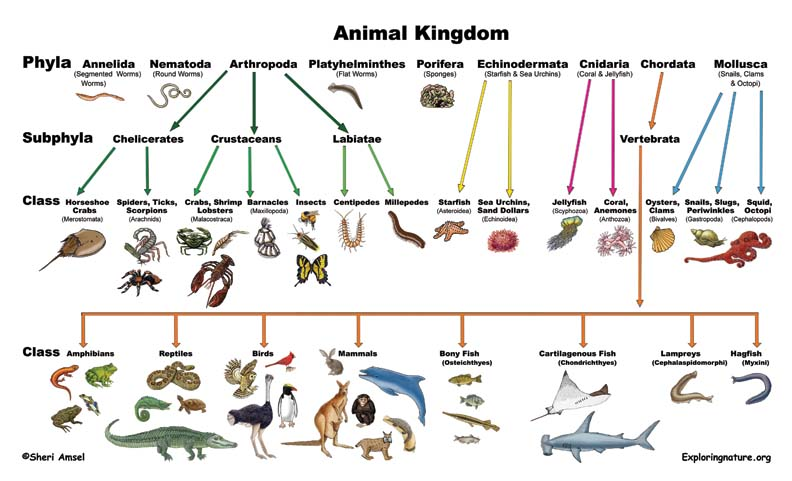
\includegraphics[width=0.7\textwidth]{figures/animal_classification}
  \caption{Classification of animals. The image is extracted from Exploring Nature.}
  \label{fig:animal_classification}
\end{figure}

\FloatBarrier

The input data for a classification task is composed by a collection of records, the dataset. In the same time, each record, also known as an instance, is composed by a set attributes. From all these attributes there is one considered special, which is called the target attribute or the class label. Regular attributes can be both discrete or continuous values. For the values signed for the class label, however, they must be discrete. This characteristic is what distinguishes classification form regression. Table \ref{tab:clasiffication_table} a sample dataset for animal classification into the following categories: amphibian, bird, fish or mammal.

\begin{table}[!htp]
\centering
\begin{tabular}{ |c|c|c|c|c|c|c|c| }
\hline
Common Name & Hair & Feathers & Eggs & Milk & Aquatic & Legs & Class Label \\ \hline
antelope & Yes & No & No & No & No & 4 & mammal \\ \hline
catfish & No & No & Yes & No & Yes & 0 & fish \\ \hline
dolphin & No & No & No & Yes & Yes & 0 & mammal \\ \hline
dove & No & Yes & Yes & No & No & 2 & bird \\ \hline
duck & No & Yes & Yes & No & Yes & 2 & bird \\ \hline
elephant & Yes & Yes & No & Yes & No & 4 & mammal \\ \hline
flamingo & Yes & Yes & Yes & No & No & 2 & bird \\ \hline
frog & No & No & Yes & No & Yes & 4 & amphibian \\ \hline
fruit bat & Yes & No & No & Yes & No & 2 & mammal \\ \hline
gull & No & Yes & Yes & No & Yes & 2 & bird \\ \hline
herring & No & No & Yes & No & Yes & 0 & fish \\ \hline
kiwi & No & No & Yes & No & No & 2 & bird \\ \hline
lark & No & Yes & Yes & No & No & 2 & bird \\ \hline
lynx & Yes & No & No & Yes & No & 4 & mammal \\ \hline
mole & Yes & No & No & Yes & No & 4 & mammal \\ \hline
mongoose & Yes & No & No & Yes & No & 4 & mammal \\ \hline
newt & No & No & Yes & No & Yes & 4 & amphibian \\ \hline
\end{tabular}
\label{tab:clasiffication_table}
\caption{Animal kingdom dataset.}
\end{table}

Definition (Classification). Classification is the task of learning a target function f that maps each attribute set x to one of the predefined class labels y.

The target function is also known informally as a classification model.

A classification model is useful for the following purposes:

\begin{itemize}
\item \textbf{Descriptive Modeling:} A classification model can serve as an explanatory tool to distinguish between objects of different classes.

\item \textbf{Predictive Modeling:} A classification model can also be used to predict the class label of unknown records. As shown in Figure \ref{fig:classification_task}, a classification model can be treated as a black box that automatically assigns a class label when presented with the attribute set of an unknown record.
\end{itemize}

\begin{figure}[!htp]
  \center
  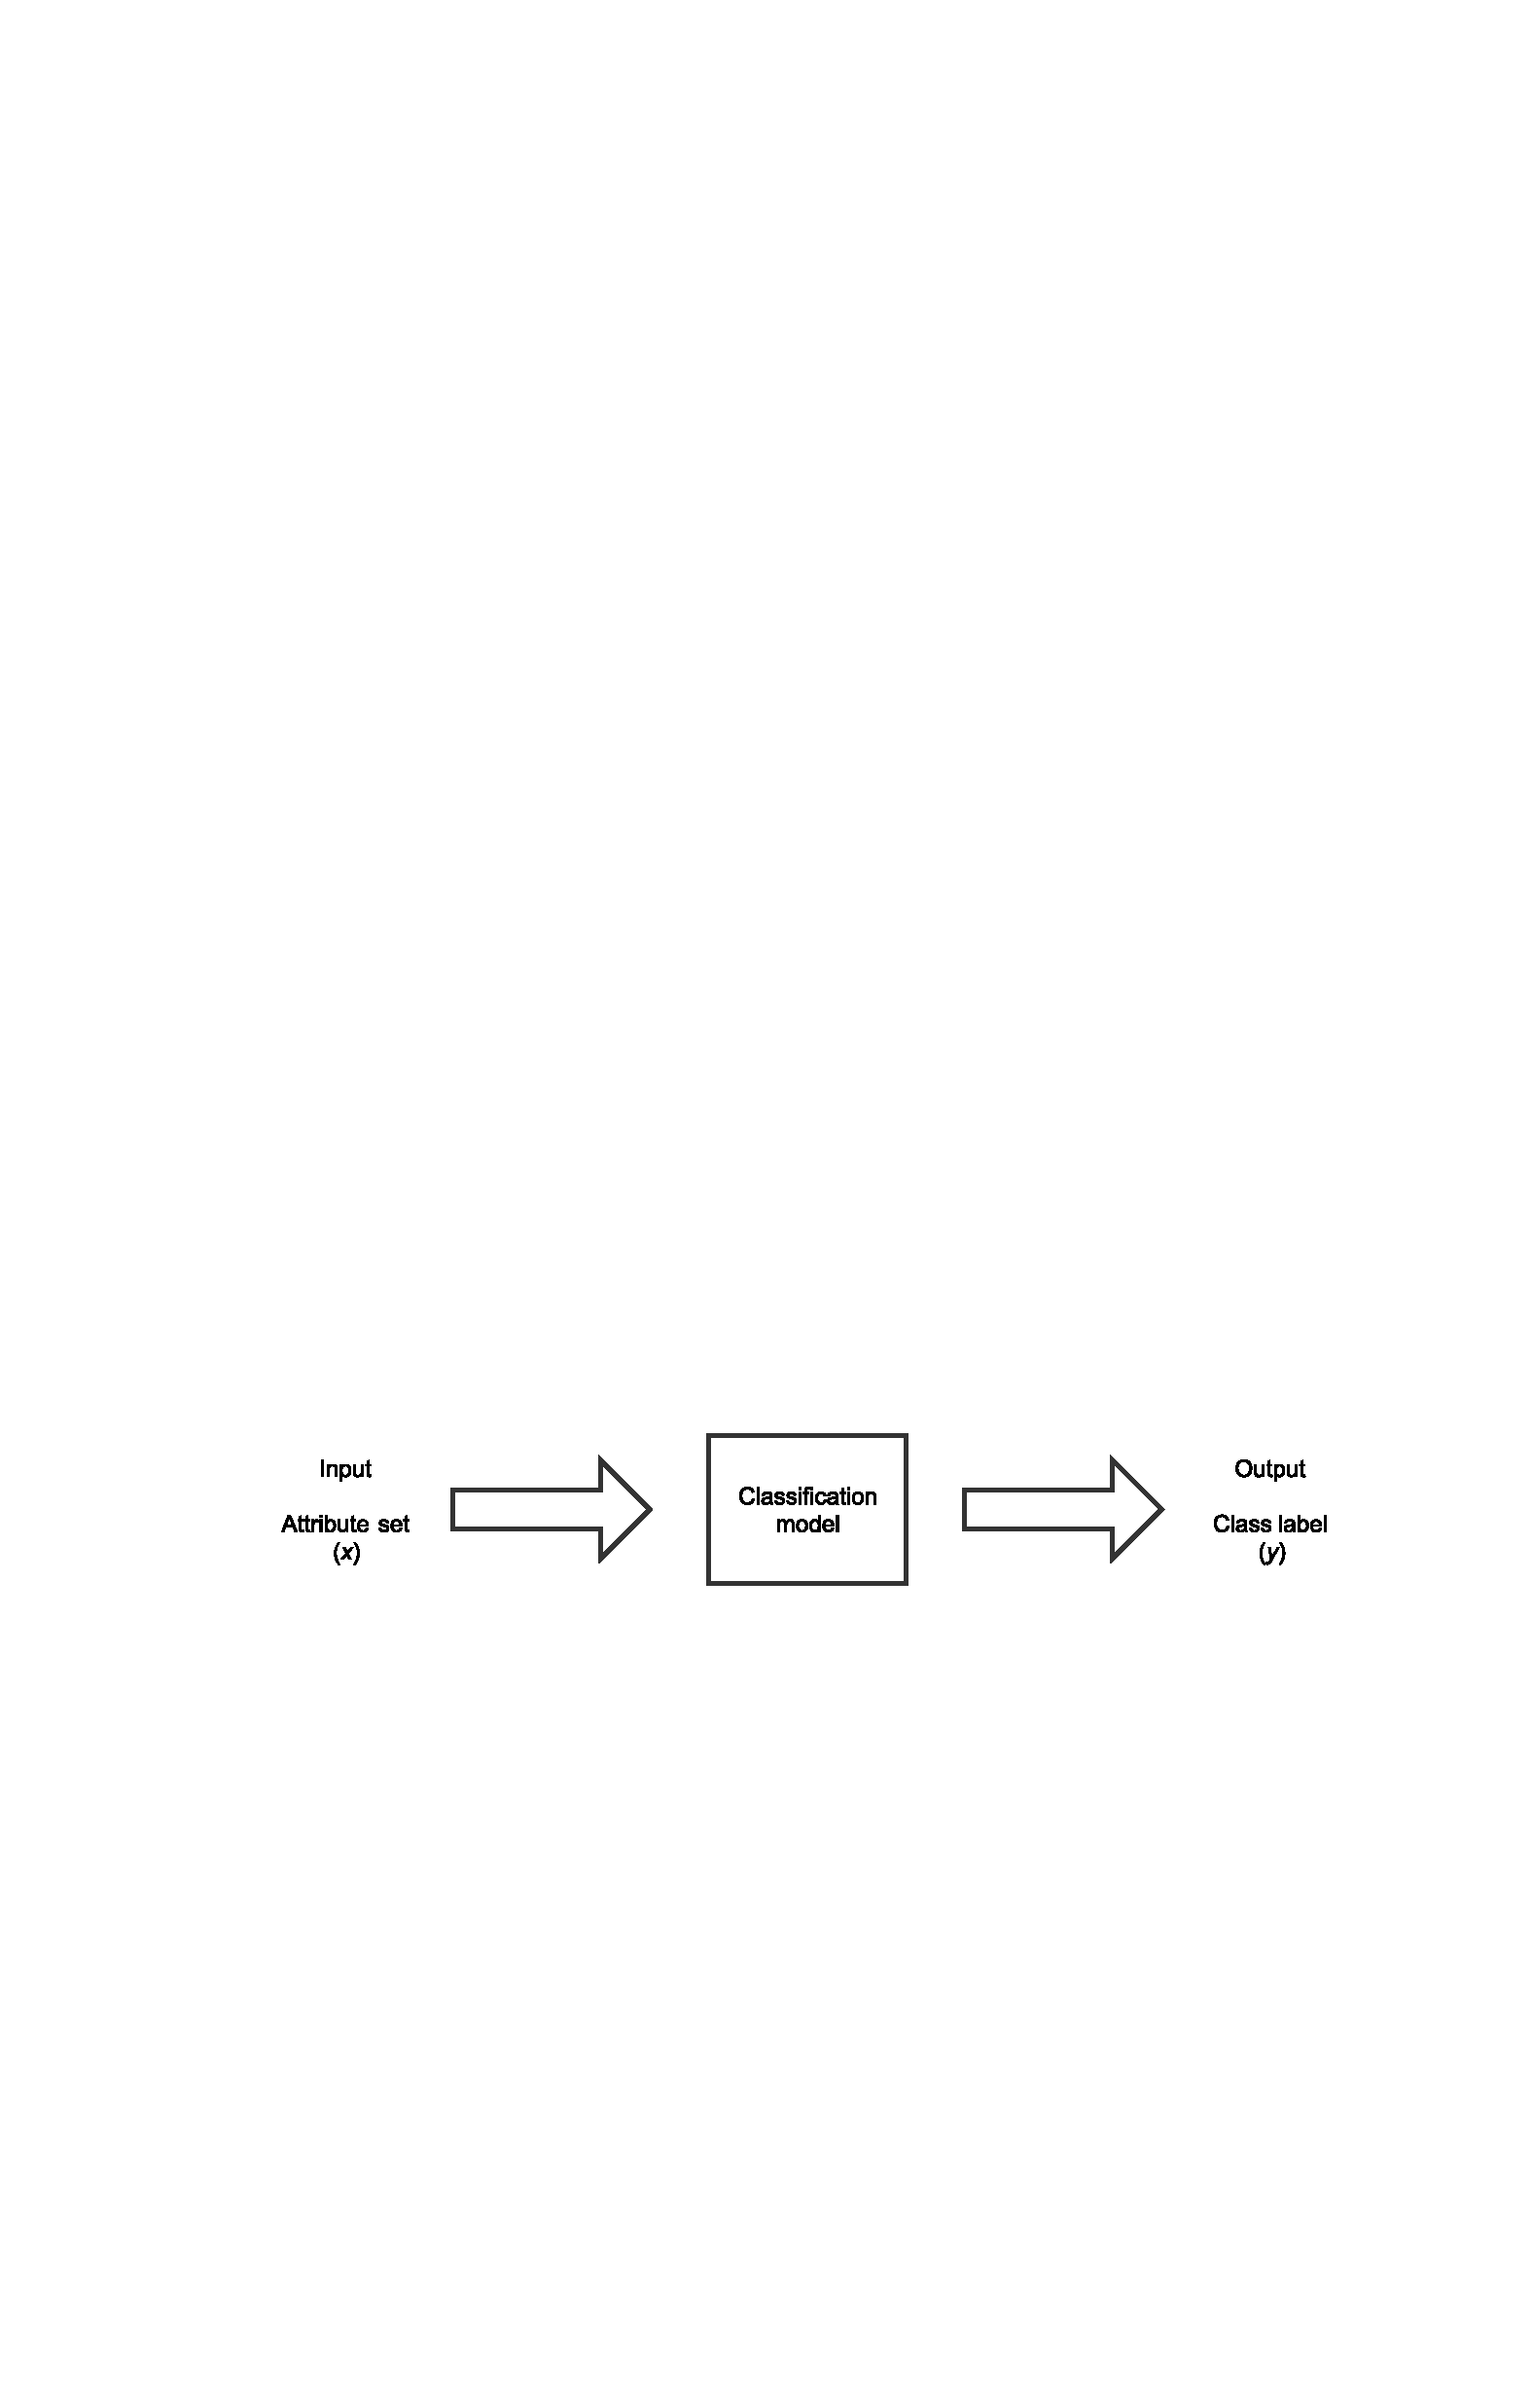
\includegraphics[width=0.7\textwidth]{figures/classification}
  \caption{Classification as a task of mapping a set attributes $x$ into its fitting class label $y$.}
  \label{fig:classification_task}
\end{figure}

\FloatBarrier

Classification techniques are most suited for predicting or describing data sets with binary or nominal categories. They are less effective for ordinal categories, because they do not consider the implicit order among the categories. Other forms of relationships, such as the subclass–superclass relationships among categories.

\section{Support Vector Machine}

There are four main advantages: Firstly it has a regularisation parameter, which makes the user think about avoiding over-fitting. Secondly it uses the kernel trick, so you can build in expert knowledge about the problem via engineering the kernel. Thirdly an SVM is defined by a convex optimisation problem (no local minima) for which there are efficient methods (e.g. SMO). Lastly, it is an approximation to a bound on the test error rate, and there is a substantial body of theory behind it which suggests it should be a good idea.
The disadvantages are that the theory only really covers the determination of the parameters for a given value of the regularisation and kernel parameters and choice of kernel. In a way the SVM moves the problem of over-fitting from optimising the parameters to model selection. Sadly kernel models can be quite sensitive to over-fitting the model selection criterion \cite{cawley2010over}

--------------------

SVMs are a new promising non-linear, non-parametric classification tech- nique, which already showed good results in the medical diagnostics, optical character recognition, elec- tric load forecasting and other fields.

Suitable for binary classification tasks.

The advantages of the SVM technique can be summarised as follows \cite{auria2008support}:

\begin{enumerate}
\item By introducing the kernel, SVMs gain flexibility in the choice of the form of the threshold separating solvent from insolvent companies, which needs not be linear and even needs not have the same func- tional form for all data, since its function is non-parametric and operates locally. As a consequence they can work with financial ratios, which show a non-monotone relation to the score and to the probability of default, or which are non-linearly dependent, and this without needing any specific work on each non-monotone variable.
\item Since the kernel implicitly contains a non-linear transformation, no assumptions about the functional form of the transformation, which makes data linearly separable, is necessary. The transformation oc- curs implicitly on a robust theoretical basis and human expertise judgement beforehand is not needed.
\item SVMs provide a good out-of-sample generalization, if the parameters C and r (in the case of a Gaussian kernel) are appropriately chosen. This means that, by choosing an appropriate generalization grade, SVMs can be robust, even when the training sample has some bias
\item SVMs deliver a unique solution, since the optimality problem is convex. This is an advantage compared to Neural Networks, which have multiple solutions associated with local minima and for this reason may not be robust over different samples.
\item With the choice of an appropriate kernel, such as the Gaussian kernel, one can put more stress on the similarity between companies, because the more similar the financial structure of two companies is, the higher is the value of the kernel. Thus when classifying a new company, the values of its financial ratios are compared with the ones of the support vectors of the training sample which are more similar to this new company. This company is then classified according to with which group it has the greatest similarity.
\end{enumerate}

--------------------------

Furthermore, $K(\bm{x}i, \bm{x}j ) \equiv \phi(\bm{x}_i)^T \phi(\bm{x}_j)$ is called the kernel function.

four basic kernels \cite{hsu2003practical}:

\begin{itemize}
\item \textbf{Linear:} $K(\bm{x}_i,\bm{x}_j) = \bm{x}^T_i \bm{x}_j$.
\item \textbf{Polynomial:} $K(\bm{x}_i,\bm{x}_j) = (\gamma \bm{x}^T_i \bm{x}_j + r)^d, \gamma > 0$.
\item \textbf{Radial Basis Function (RBF):} $K(\bm{x}_i,\bm{x}_j) = \exp(−\gamma \lVert \bm{x}_i − \bm{x}_j \rVert ^2),\gamma > 0$.
\item \textbf{Sigmoid:} $K(\bm{x}_i,\bm{x}_j) = \tanh(\gamma \bm{x}^T_i\bm{x}_j + r)$.
\end{itemize}

Here, $\gamma$, $r$, and $d$ are kernel parameters.

--------------------------

Support vector machines (SVM) were originally designed for binary classification \cite{hsu2002comparison}.

solving multi-class SVM in one step: “all-together” methods: [25], [27] and [7]. We then compare their performance with three methods based on binary classifications: “one-against-all,” “one-against-one,” and DAGSVM [23]. Our experiments indicate that the “one-against-one” and DAG methods are more suitable for practical use than the other methods. 

--------------------------

asdasdasd \cite{berwick2003idiot}

\begin{figure}[!htp]
  \center
  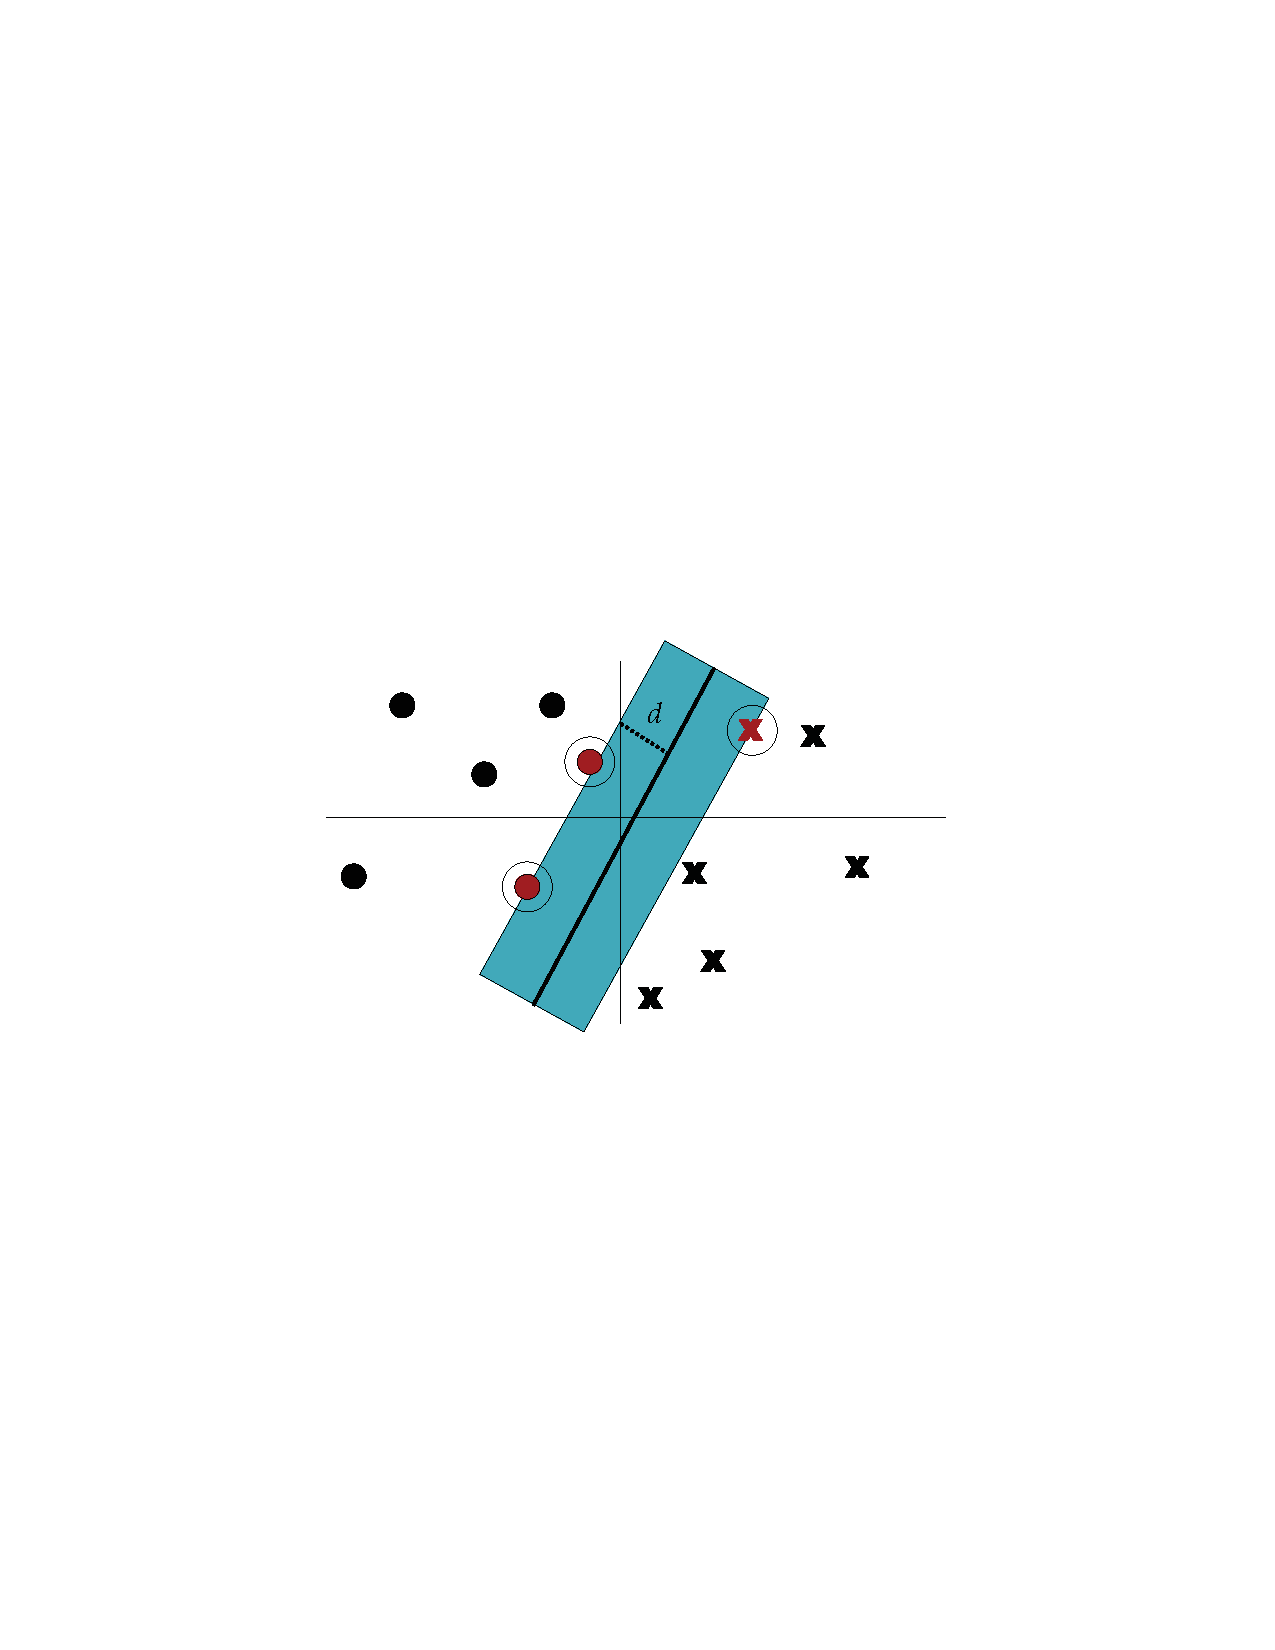
\includegraphics[width=0.6\textwidth]{figures/hyperplane}
  \caption{hyperplane}
  \label{fig:hyperplane}
\end{figure}

\section{K-Nearest Neighbor}

\section{Neural Networks}
